This chapter details Support module which includes: forum, chat and tutorials.
\section{Forum}
GATE Teamware includes forum powered by \url{http://www.jforum.net}.
The complete list of features is available at:
\url{http://www.jforum.net/features.jsp}.

The forum is envisaged to serve as the primary way for interactive support, instead of mailing list.
As with any advanced forum, users can post new messages and replies, or create new topics. 

Figure~\ref{fig:forum} depicts the main forum page with list of available forums. 

Feel free to use this forum to post any particular questions, report bugs and suggest any new features for the GATE Teamware.
\begin{figure}[hb!]
\centering
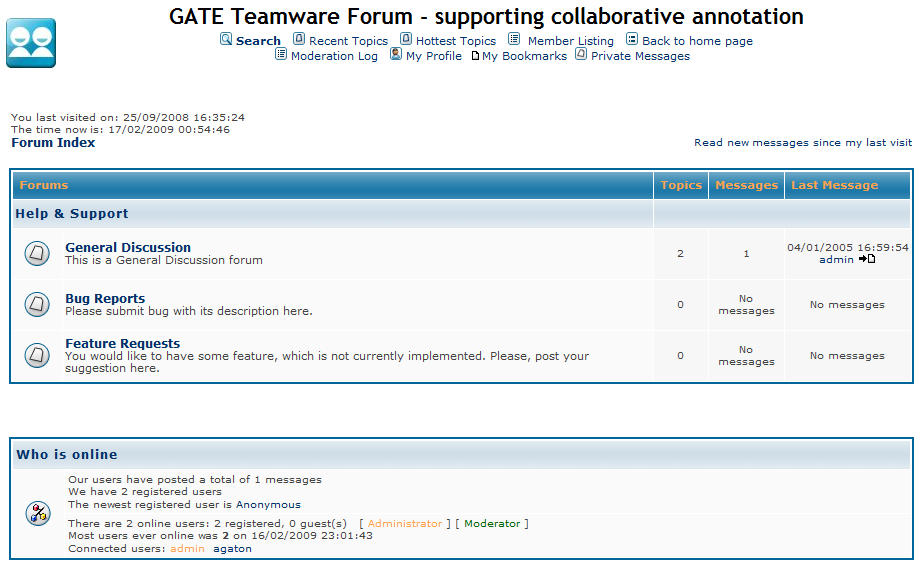
\includegraphics[scale=0.4]{forum}
\caption{Forum home page}
\label{fig:forum}
\end{figure}

Users with \emph{administrator} role can change forum settings and create new forums and categories. This is accomplished through the adiministration panel shown in Figure~\ref{fig:forumadmin} below.

\begin{figure}
\centering
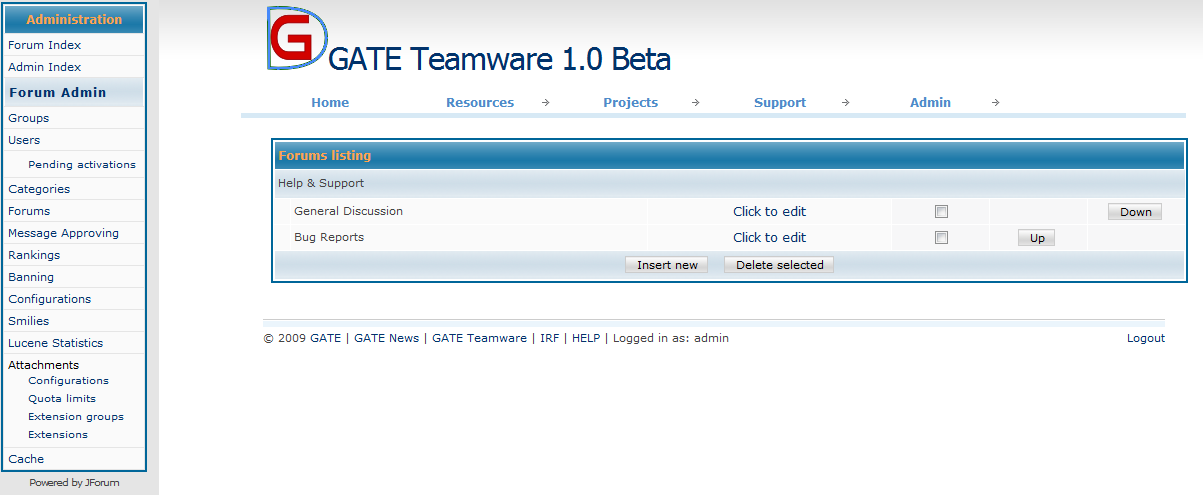
\includegraphics[scale=0.4]{forumadmin}
\label{fig:forumadmin}
\end{figure}

\section{Chat}

Chat is still in experimental phase. Currently, this service is very basic, as shown in Figure~\ref{fig:chat}).
\begin{figure}[hb!]
\centering
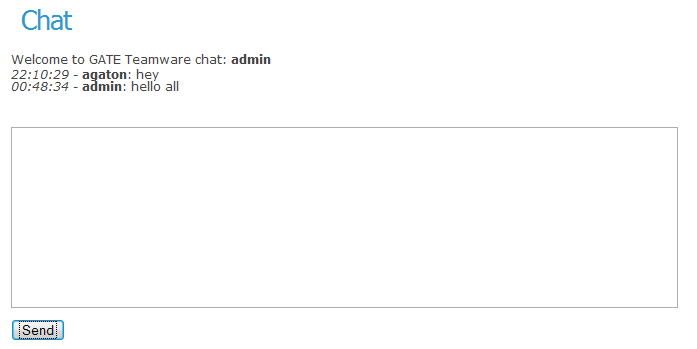
\includegraphics[scale=0.4]{chat}
\caption{Chat Window}
\label{fig:chat}
\end{figure}

Message is broadcasted to all logged users. This is implemented with the idea to see if such functionality can be of interest to the users.
\section{Help}
Apart from this user guide, in this section you will find several movie tutorials which can help you to familiarise yourself with the GATE Teamware interface and functionalities.
% \begin{figure}[hb!]
% \centering
% 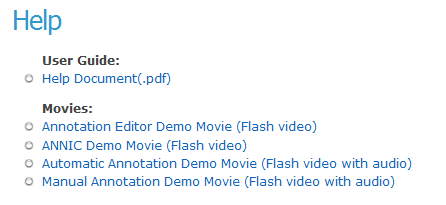
\includegraphics[scale=0.4]{help}
% \caption{Help Window}
% \label{fig:help}
% \end{figure}
